\documentclass[english]{maciarticle}

\usepackage{amsmath,amsbsy,amscd,amssymb,graphicx, epsfig,color,float}

%%%%%%%%%%%%%%%%%%%%%%%%%%%%%%%%%%%%%%%%%%%%%
\begin{document}

\title{Hierarchical Risk Parity for Cryptocurrency Portfolios: A Comparative Analysis}

\author[$\flat$]{Alan Matys}
\author[$\dag$]{Federico Martin Rodriguez}
\affil[$\flat$]{Universidad del CEMA,
\textcolor{blue} {alan.matys92@gmail.com, federico.m.rodriguez.h@gmail.com}}

\maketitle

\begin{abstract}
This article addresses portfolio construction as a budget allocation problem, balancing expected returns with risk mitigation. Traditional methods like the Critical Line Algorithm (CLA) struggle with diversification due to their sensitivity to input parameters. Hierarchical Risk Parity (HRP) offers a robust alternative by employing correlation-based clustering and hierarchical weight allocation. We evaluate HRP’s effectiveness in cryptocurrency markets, where traditional optimization methods face challenges due to high volatility and inter-asset correlations. Our findings demonstrate that HRP achieves superior diversification while maintaining computational stability, making it a compelling choice for risk-based asset allocation.
\end{abstract}

\begin{keywords}
Hierarchical Risk Parity, Risk-based asset allocation, Cryptocurrency, Portfolio Optimization
\end{keywords}

\begin{mathsubclass}
21A54 - 55P54
\end{mathsubclass}

{\thispagestyle{empty}} %DO NOT DELETE THIS LINE

%%===============================
\section{Introduction}
%%===============================

The portfolio construction problem is a constrained optimization challenge where investors allocate capital across assets while balancing expected returns against risk, defined as return deviation.

A common approach to portfolio optimization is the \textbf{Markowitz Critical Line Algorithm (CLA)}, which minimizes variance given return estimates over a defined time window. While CLA provides a theoretically optimal solution, it has notable advantages and limitations:

\begin{itemize}
    \item \textbf{Pros:} Ensures weight convergence after a finite number of steps.
    \item \textbf{Cons:} Prone to instability, high asset concentration, and potential underperformance.
\end{itemize}

Additionally, CLA relies on inverting the variance-covariance matrix, a process that can become numerically unstable depending on its structure.

Risk-based asset allocation methods aim to mitigate these challenges. Among them, \textbf{Hierarchical Risk Parity (HRP)} introduces a novel weighting strategy, clustering correlated assets before assigning weights. This article explores the application of \textbf{HRP in cryptocurrency markets}, leveraging its ability to enhance diversification while addressing estimation uncertainty in risk and return parameters.

%%===============================
\section{HRP Portfolio Building}
%%===============================

The \textbf{Hierarchical Risk Parity (HRP)} approach consists of three key steps:

\subsection{Hierarchical Clustering}
The first step in HRP is the construction of a hierarchical clustering structure based on asset correlations. This process begins by computing a \textbf{distance matrix} derived from the correlations of \(N\) assets.

The correlation matrix is defined as:

\[
\rho = \left( \rho_{i,j} \right)_{i,j=1,...,N}
\]

where each element \(\rho_{i,j}\) represents the correlation between asset \(X_i\) and asset \(X_j\):

\[
\rho_{i,j} = \rho[X_i, X_j].
\]

Since the correlation matrix is bounded within \([-1,1]\), its scale does not affect the clustering process.

From this correlation matrix, we construct a \textbf{distance metric} to measure the dissimilarity between asset pairs. The metric is defined as:

\[
d : (X_i, X_j) \subseteq \mathcal{B} \to \mathbb{R} \in [0, 1], \quad d_{i,j} = d[X_i, X_j] = \sqrt{\frac{1}{2}(1 - \rho_{i,j})}.
\]

where \(\mathcal{B}\) represents the Cartesian product of asset pairs.

With the previously computed distance matrix, we calculate the Euclidean distances between the columns of the matrix:

\[
\tilde{d} : (D_i, D_j) \subseteq \mathcal{B} \to \mathbb{R} \in [0, \sqrt{N}], \quad \tilde{d}_{i,j} = \tilde{d}[D_i, D_j] = \sqrt{\sum_{n=1}^N (d_{n,i} - d_{n,j})^2}.
\]

Finally, assets are grouped based on the final matrix using a linkage criterion, determining the hierarchical structure necessary for the next steps of the HRP process.

\subsection{Quasi-Diagonalization}
In this step, the matrix is reorganized such that rows and columns are arranged so that the largest values in the distance matrix are grouped along the diagonal.

Based on the clusters identified in the previous step, we reorder the matrix so that similar assets are positioned closer together, while uncorrelated or negatively correlated assets are placed farther apart. This structured ordering allows for a clearer representation of asset relationships and improves the stability of subsequent calculations.

\subsection{Recursive Bisection}
Using the quasi-diagonalization from the previous step, we now determine the optimal portfolio allocation by applying the Inverse Variance Portfolio (IVP) method within each group. The recursive bisection process follows these steps:

\begin{itemize}
    \item First, allocate weights to each major group identified in the clustering step.
    \item Then, recursively divide the assigned weights within each subgroup.
    \item Continue subdividing until further partitioning is no longer possible.
\end{itemize}

This ensures a stable and diversified allocation while avoiding over-concentration in specific assets.

%%===============================
\section{Results and Evaluation Methodology}
%%===============================

The proposed method is tested against traditional portfolio allocation techniques, including the Inverse Variance Portfolio (IVP) and the Minimum Variance Portfolio (MVP), as well as against holding BTC and ETH for the entire backtesting period. The backtesting period spans from  \textbf{January 1, 2021, to December 31, 2023}.

\subsection{Comparison Scenarios}
The methodology is assessed under two distinct scenarios:

\begin{itemize}
    \item \textbf{Static Portfolio Allocation}: Weights are assigned once at the beginning of the backtesting period without rebalancing.
    \item \textbf{Monthly Rebalancing}: The best-performing method from the static scenario is compared with the three methodologies under a monthly rebalancing strategy, incorporating a transaction cost rate of 0.1\% per trade.
\end{itemize}

\subsection{Evaluation Metrics}
Performance is evaluated using the following metrics:

\begin{itemize}
    \item \textbf{Total Return (\%)}: The cumulative percentage gain or loss over the backtesting period.
    \item \textbf{Annualized Volatility (\%)}: Measures the standard deviation of returns on an annual basis.
    \item \textbf{Sharpe Ratio}: Evaluates risk-adjusted returns by comparing excess returns over the risk-free rate relative to volatility. In this analysis, the risk-free rate is assumed to be 0.
    \item \textbf{Sortino Ratio}: Similar to the Sharpe Ratio but only considers downside risk.
    \item \textbf{Maximum Drawdown (\%)}: The largest peak-to-trough decline in portfolio value during the period.
    \item \textbf{Calmar Ratio}: The return-to-risk measure comparing total return to maximum drawdown.
\end{itemize}

%%===============================
\subsection{Final Results}
%%===============================

\subsubsection{Static Portfolio Allocation Results}

\begin{figure}[H]
    \centering
    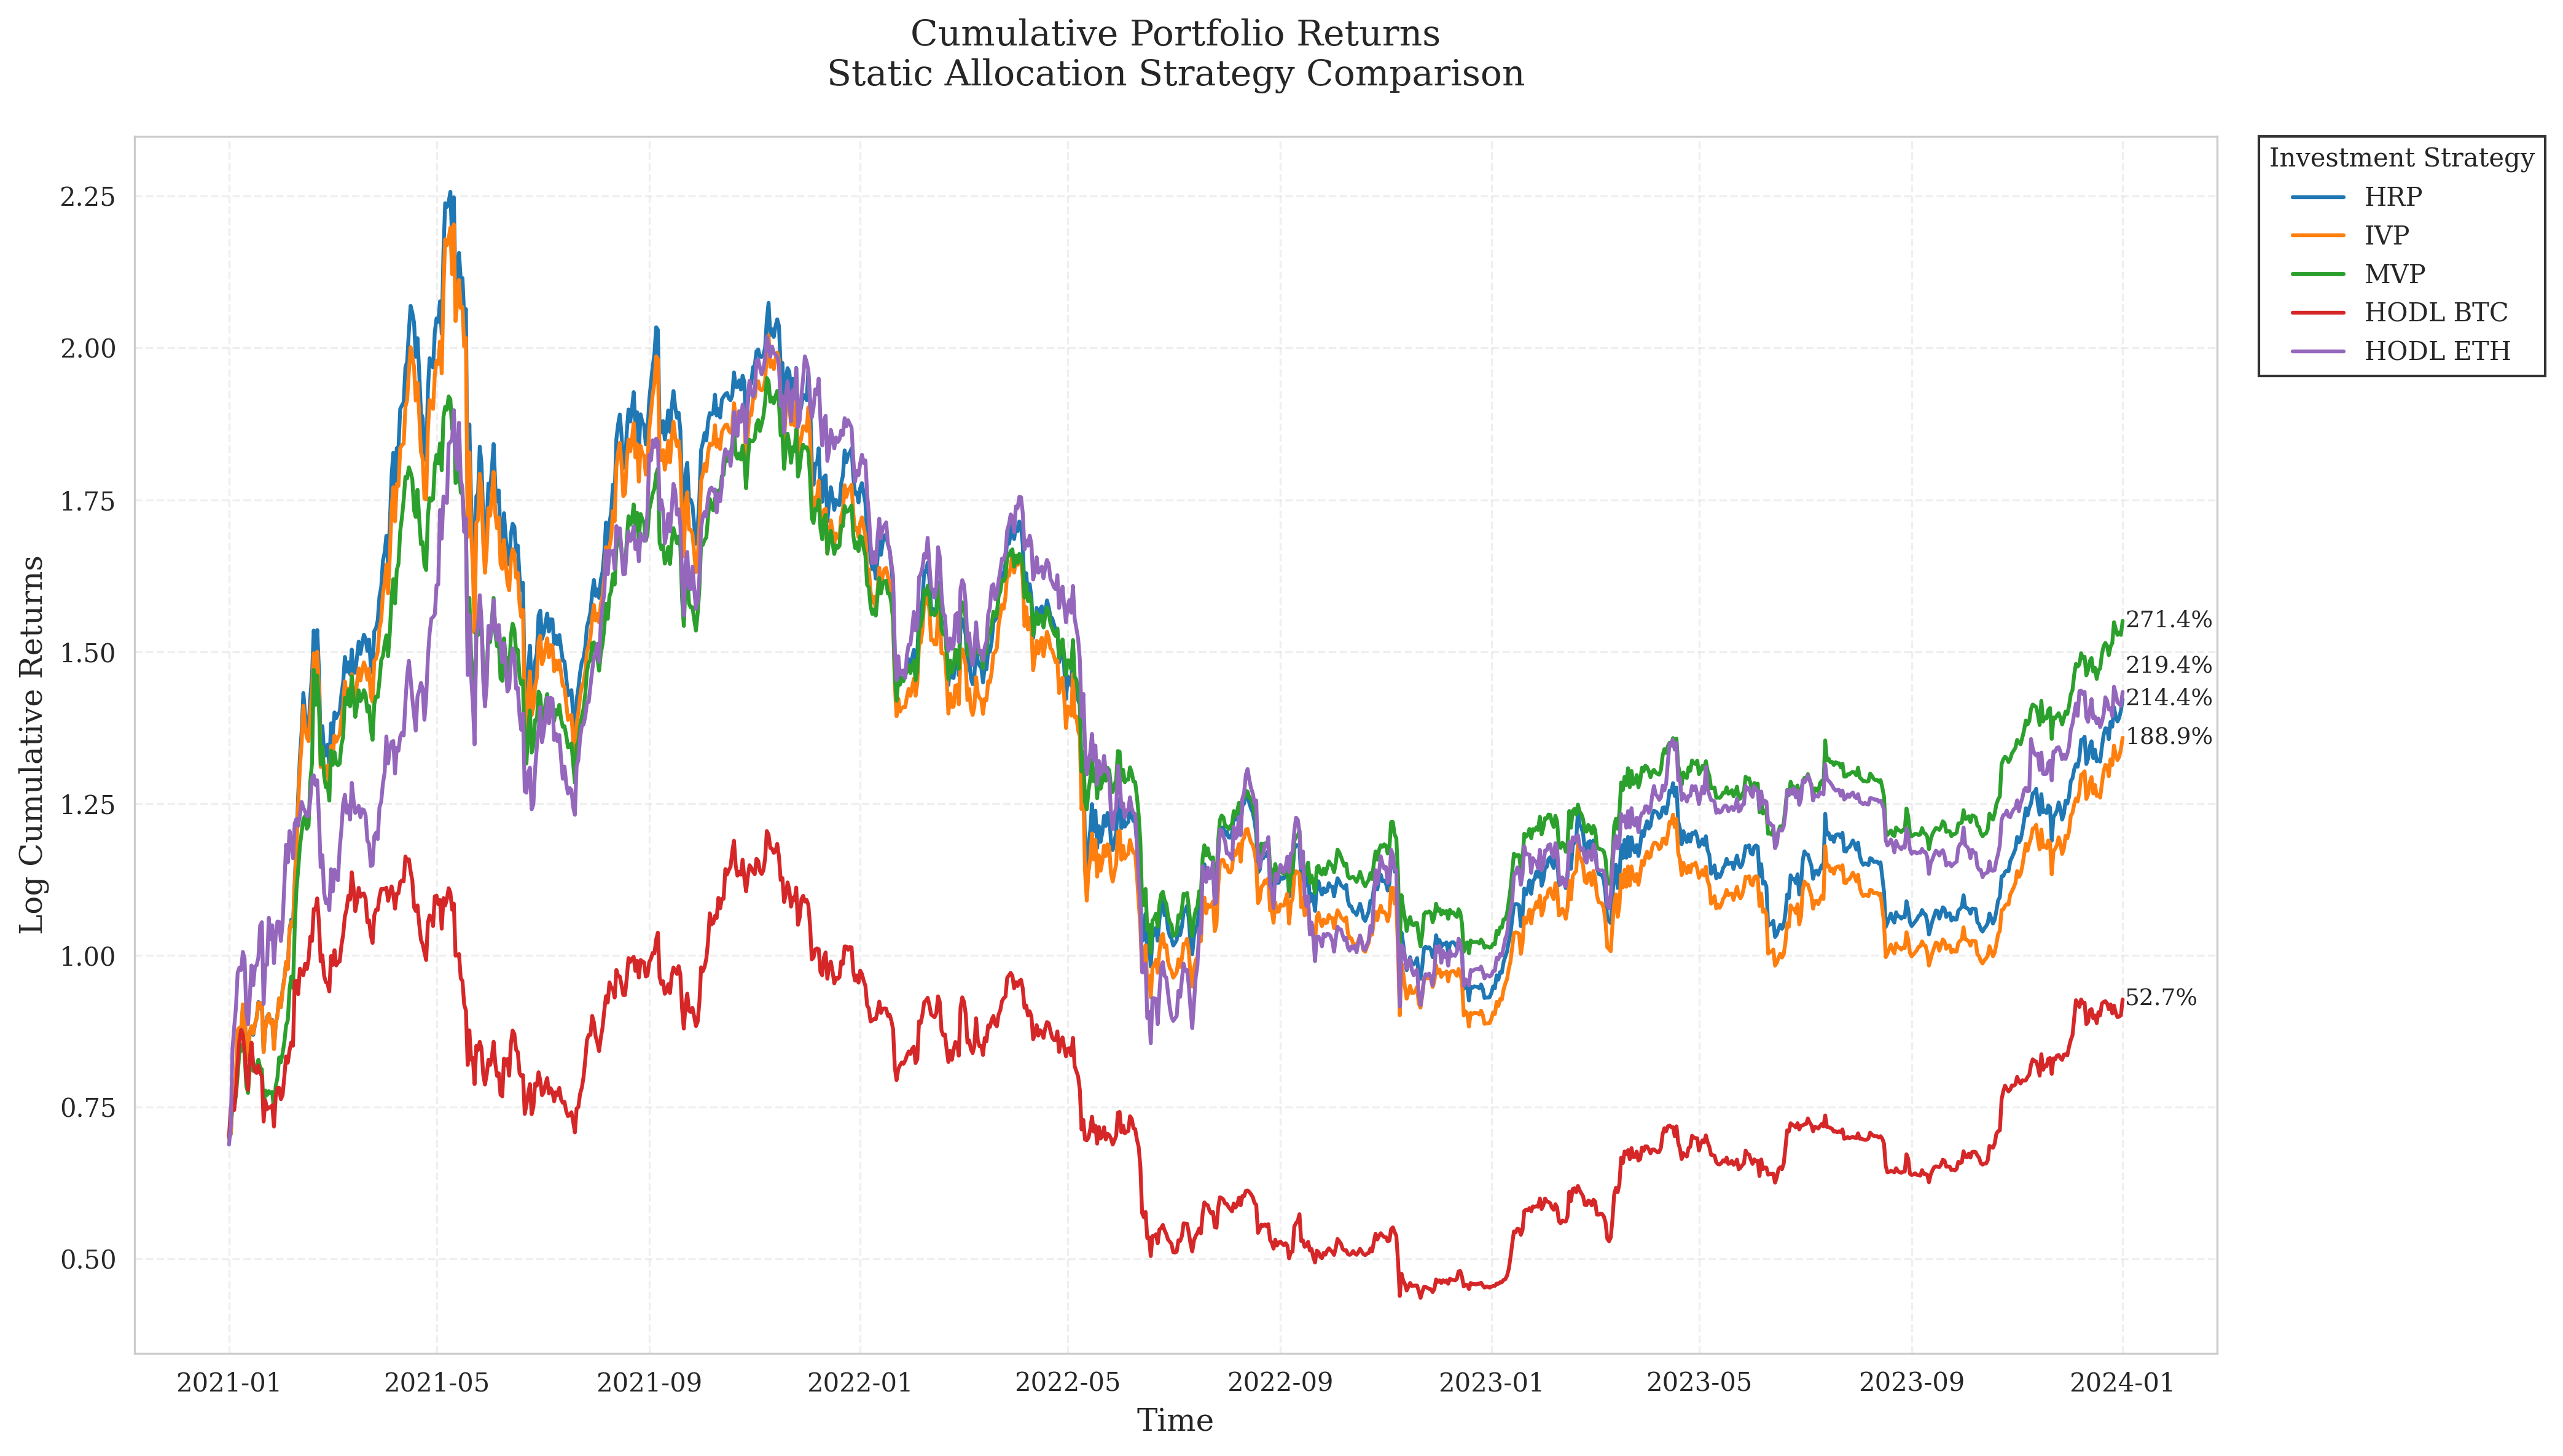
\includegraphics[width=0.8\textwidth]{static_cumulative_returns.png}
    \caption{Cumulative Returns for Static Portfolio Allocation.}
    \label{fig:static_cum_returns}
\end{figure}

\vspace{-0.5cm}

\begin{table}[H]
    \centering
    \renewcommand{\arraystretch}{1.1}
    \small % Reduce font size
    \caption{Performance Metrics for Static Portfolio Allocation}
    \begin{tabular}{|l|c|c|c|c|c|c|}
    \hline
    Portfolio & Total Return (\%) & Ann. Volatility (\%) & Sharpe Ratio & Sortino Ratio & Max Drawdown (\%) & Calmar Ratio \\
    \hline
    HRP & 214.45 & 82.17 & 0.88 & 0.82 & -82.21 & 0.57 \\
    IVP & 188.86 & 82.07 & 0.85 & 0.79 & -82.42 & 0.51 \\
    MVP & 271.45 & 70.51 & 0.97 & 0.98 & -71.38 & 0.77 \\
    HODL BTC & 52.75 & 64.86 & 0.54 & 0.57 & -76.63 & 0.20 \\
    HODL ETH & 219.39 & 84.68 & 0.88 & 0.91 & -79.30 & 0.60 \\
    \hline
    \end{tabular}
\end{table}

\subsubsection{Monthly Rebalancing Results}

\begin{figure}[H]
    \centering
    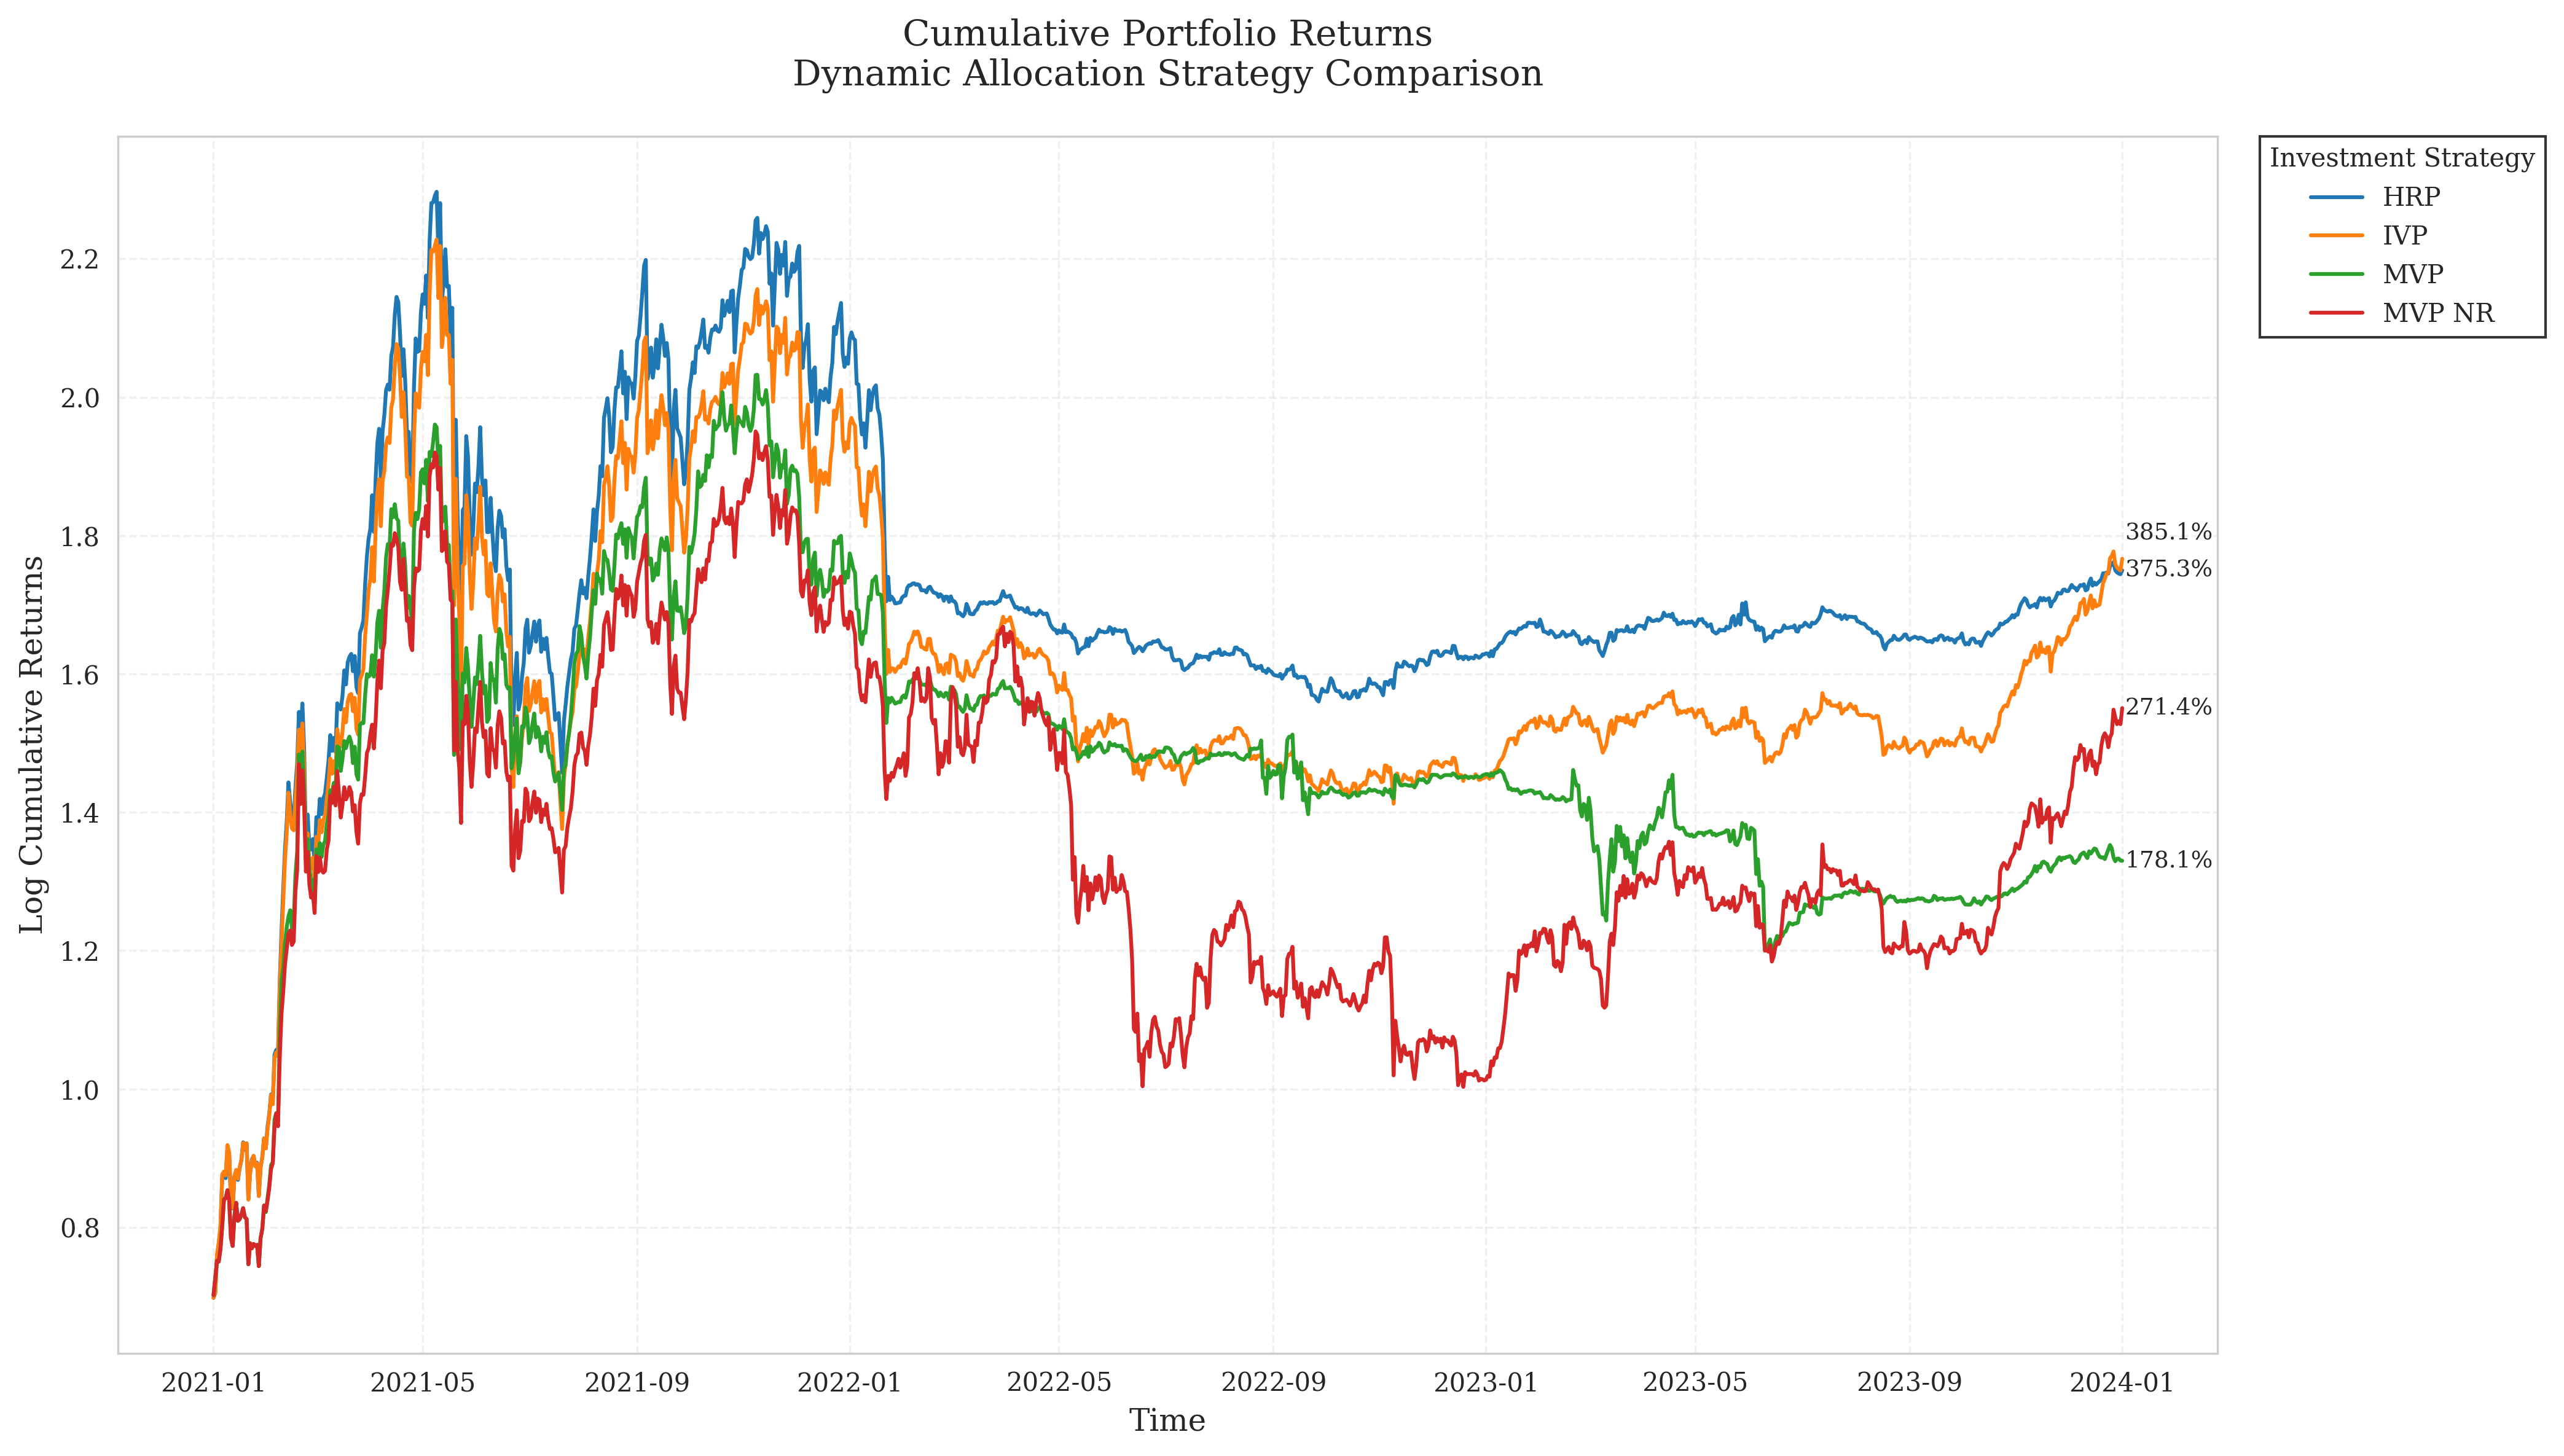
\includegraphics[width=0.8\textwidth]{rebalancing_cumulative_returns.png}
    \caption{Cumulative Returns for Monthly Rebalancing.}
    \label{fig:rebalance_cum_returns}
\end{figure}

\vspace{-0.5cm}

\begin{table}[H]
    \centering
    \renewcommand{\arraystretch}{1.1}
    \small % Reduce font size
    \caption{Performance Metrics for Monthly Rebalancing}
    \begin{tabular}{|l|c|c|c|c|c|c|}
    \hline
    Portfolio & Total Return (\%) & Ann. Volatility (\%) & Sharpe Ratio & Sortino Ratio & Max Drawdown (\%) & Calmar Ratio \\
    \hline
    MVP NR & 271.45 & 70.51 & 0.97 & 0.98 & -71.38 & 0.77 \\
    HRP & 375.32 & 68.41 & 1.11 & 1.09 & -63.17 & 1.08 \\
    IVP & 385.06 & 68.92 & 1.12 & 1.06 & -64.28 & 1.08 \\
    MVP & 178.09 & 60.87 & 0.87 & 0.90 & -65.31 & 0.62 \\
    \hline
    \end{tabular}
\end{table}

%%===============================
\section{Conclusion \& Future Research}
%%===============================

\subsection{Conclusion}

\textbf{Diversification}: For portfolios without rebalancing, capital allocation is more evenly distributed. However, for rebalanced portfolios, allocations become more concentrated over time.

\textbf{Rebalancing}: In MVP, each rebalancing step can lead to significant changes in allocation, resulting in high transaction costs that reduce returns.

\subsection{Future Research}

\textbf{Denoising}: Addressing noise caused by small eigenvalues in the correlation matrix.

\textbf{Denoting}: Adjusting for market-wide correlation shocks by filtering out systemic movements.

%%===============================
\section*{Acknowledgements}
%%===============================

We thank all the Ucema Quant professors and staff, especially Manuel Maurette, Emiliano Delfau and Pablo Martin Gechidjian. Finally, we extend our gratitude to Marcos López de Prado for his contributions to the field through his bibliography.

\begin{thebibliography}{9}

\bibitem{lopez2016}
López de Prado, M. (2016). \textit{Building Diversified Portfolios that Outperform Out-of-Sample}. Journal of Portfolio Management. \texttt{https://doi.org/10.3905/jpm.2016.42.4.059}.

\bibitem{lopez2018}
López de Prado, M. (2018). \textit{Advances in Financial Machine Learning}. John Wiley \& Sons.

\bibitem{lopez2020}
López de Prado, M. (2020). \textit{Machine Learning for Asset Managers}. Cambridge University Press.

\end{thebibliography}

\end{document}